\setcounter{section}{1}
\section{CÔNG THỨC XÁC SUẤT TOÀN PHẦN VÀ CÔNG THỨC BAYES}
%%%%%%%%%%%%%%%%
\subsection{Trọng tâm kiến thức}
\begin{tomtat}
\subsubsection{Công thức xác suất toàn phần}
\begin{boxdn}
Cho hai biến cố $A$ và $B$ là hai biến cố tùy ý. Khi đó
$$\mathrm{P}(A)=\mathrm{P}(B)\cdot \mathrm{P}(A|B)+\mathrm{P}(\overline{B})\cdot \mathrm{P}(A|\overline{B}).$$
Công thức trên được gọi là công thức xác suất toàn phần.
\end{boxdn}
\subsubsection{Công thức Bayes}
\begin{boxdn}
Cho hai biến cố $A$ và $B$ với $\mathrm{P}(A)>0$. Khi đó
$$\mathrm{P}\left(B|A\right)=\dfrac{\mathrm{P}(B)\cdot\mathrm{P}\left(A|B\right)}{\mathrm{P}(A)}.$$
\end{boxdn}
\begin{note}
Công thức Bayes còn được viết dưới dạng 
$$\mathrm{P}(B | A)=\dfrac{\mathrm{P}(B) \cdot \mathrm{P}(A \mid B)}{\mathrm{P}(B)\cdot \mathrm{P}(A | B)+\mathrm{P}\left(\overline{B}\right)\cdot \mathrm{P}\left(A | \overline{B}\right)}.$$
\end{note}
\end{tomtat}
%%%%%%%%%%%%%%
\subsection{Các dạng bài tập}
\setcounter{dang}{0}
\begin{dang}{Tính xác suất theo công thức xác suất toàn phần}
	Với hai biến cố $A$ và $B$ tùy ý thì
	$\mathrm{P}(A)=\mathrm{P}(B)\cdot\mathrm{P}(A|B)+\mathrm{P}(\overline{B})\cdot\mathrm{P}(A|\overline{B}).$
\end{dang}
%----------------------------
\subsubsection{Ví dụ minh hoạ}
\begin{vd}%[2D5H2-2]
	Cho hai biến cố $A$, $B$ với $\mathrm{P}(B)=0{,}6$; $\mathrm{P}(A|B) =0{,}7$ và $\mathrm{P}\left(A|\overline{B}\right)=0{,}4$. Tính $\mathrm{P}(A)$
	\loigiai{
		Ta có $\mathrm{P}\left(\overline{B}\right)= 1- \mathrm{P}(B) = 1-0{,}6 = 0{,}4$.\\
		Áp dụng công thức xác suất toàn phần, ta có
		\[\mathrm{P}(A) = \mathrm{P}(A|B)\cdot \mathrm{P}(B) + \mathrm{P}\left(A|\overline{B}\right)\cdot \mathrm{P}\left(\overline{B}\right)= 0{,}7\cdot 0{,}6 + 0{,}4\cdot 0{,}4=0{,}58.\]
	}
\end{vd}
\begin{vd}%[2D5H2-2]
	Trong một kì thi tốt nghiệp trung học phổ thông, một tỉnh X có $80 \%$ học sinh lựa chọn tổ hợp A00 (gồm các môn Toán, Vật lí, Hoá học). Biết rằng, nếu một học sinh chọn tổ hợp A00 thì xác suất để học sinh đó đỗ đại học là 0{,}6; còn nếu một học sinh không chọn tổ hợp A00 thì xác suất để học sinh đó đỗ đại học là 0{,}7. Chọn ngẫu nhiên một học sinh của tỉnh X đã tốt nghiệp trung học phổ thông trong kì thi trên. Tính xác suất để học sinh đó đỗ đại học.
	\loigiai{Gọi $A$ là biến cố: \lq \lq Học sinh đó chọn tổ hợp A00\rq \rq~; $B$ là biến cố: \lq \lq Học sinh đó đỗ đại học\rq \rq.\\
		Ta cần tính $\mathrm{P}(B)$. Theo công thức xác suất toàn phần, ta cần biết: $\mathrm{P}(A), \mathrm{P}(\overline{A}), \mathrm{P}(B \mid A)$ và $\mathrm{P}(B \mid \overline{A})$.\\
		Ta có: $\mathrm{P}(A)=0{,}8; \mathrm{P}(\overline{A})=1-\mathrm{P}(A)=1-0{,}8=0{,}2$.\\
		$\mathrm{P}(B \mid A)$ là xác suất để một học sinh đỗ đại học với điều kiện học sinh đó chọn tổ hợp $A 00$ \\$\Rightarrow \mathrm{P}(B \mid A)=0{,}6$.\\
		$\mathrm{P}(B \mid \overline{A})$ là xác suất để một học sinh đỗ đại học với điều kiện học sinh đó không chọn tổ hợp $\mathrm{A} 00$\\$ \Rightarrow \mathrm{P}(B \mid \overline{A})=0{,}7$.\\
		Thay vào công thức xác suất toàn phần ta được:$$\mathrm{P}( B)={\mathrm{P}(A) \cdot \mathrm{P}(B \mid A)+\mathrm{P}(\overline{A}) \cdot \mathrm{P}(B \mid \overline{A})}={0{,}8 \cdot 0{,}6+0{,}2 \cdot 0{,}7} = 0{,}62.$$}
\end{vd}
\begin{vd}%[2D5H2-2]
	\immini{
		Số khán giả đến xem buổi biểu diễn ca nhạc ngoài trời phụ thuộc vào thời tiết. Giả sử, nếu trời không mưa thì xác suất để bán hết vé là $0{,}9$; còn nếu trời mưa thì xác suất để bán hết vé chỉ là $0{,}4$. Dự báo thời tiết cho thấy xác suất để trời mưa vào buổi biểu diễn là $0{,}75$. Nhà tổ chức sự kiện quan tâm đến xác suất để bán được hết vé là bao nhiêu.\\
			Gọi $A$ là biến cố \lq \lq Trời mưa\rq \rq~và $B$ là biến cố \lq \lq Bán hết vé\rq \rq~trong tình huống.
		\begin{listEX}
			\item Tính $\mathrm{P}(A), \mathrm{P}(\overline{A}), \mathrm{P}(B \mid A), \mathrm{P}(B \mid \overline{A})$.
			\item Tính xác suất để nhà tổ chức sự kiện bán hết vé.
		\end{listEX}
	}{	\includegraphics[width=8cm,height=6cm]{images/im2D5-2-1.png}}
	\loigiai{
		\begin{listEX}
			\item $\mathrm{P}(A)=0{,}75$; $\mathrm{P}(\overline{A})=1-\mathrm{P}(A)=0{,}25$; $\mathrm{P}(B\mid A)=0{,}4$; $\mathrm{P}(B\mid \overline{A})=0{,}9$.
			\item 	Ta có $\mathrm{P}(B)= \mathrm{P}(A) \cdot \mathrm{P}(B \mid A)+\mathrm{P}(\overline{A}) \cdot \mathrm{P}(B \mid \overline{A}) = 0{,}75\cdot 0{,}4 +0{,}25\cdot 0{,}9=0{,}525$.
	\end{listEX}}
\end{vd}
\begin{vd}%[2D5H2-2]
	Một hộp có $60$ viên bi màu xanh và $40$ viên bi màu đỏ; các viên bi có kích thước và khối lượng như nhau. Sau khi thống kê, người ta thấy: có $50\%$ số viên bi màu xanh có dán nhãn và $75\%$ số viên bi màu đỏ có dán nhãn; những viên bi còn lại không có dán nhãn.
	\begin{listEX}
		\item Chọn số thích hợp cho $\boxed{?}$ trong bảng (đơn vị: viên bi).
		\begin{center}
			\begin{tabular}{|c|C{3cm}|C{3cm}|}
				\hline
				\diaghead{Dán nhãn Màu bi}{\normalsize Màu bi}{\normalsize Dán nhãn} & Có dán nhãn & Không dán nhãn \\
				\hline
				Đỏ & $\boxed{?}$ & $\boxed{?}$ \\
				\hline
				Xanh & $\boxed{?}$ & $\boxed{?}$\\
				\hline
			\end{tabular}
		\end{center}
		\item Lấy ra ngẫu nhiên một viên bi trong hộp. Sử dụng công thức xác suất toàn phần, tính xác suất để viên bi được lấy ra có dán nhãn.
	\end{listEX}
	\loigiai{
		\begin{listEX}
			\item Số viên bi màu đỏ có dán nhãn là $75\%\cdot 40 = 30$ (viên bi).\\
			Số viên bi màu xanh có dãn nhẫn là $50\%\cdot 60 = 30$ (viên bi).\\
			\begin{center}
				\begin{tabular}{|c|C{2.75cm}|C{2.75cm}|}
					\hline
					\diaghead{Dán nhãn Màu bi}{\normalsize Dán nhãn}{\normalsize Màu bi} & Có dán nhãn & Không dán nhãn \\
					\hline
					Đỏ & $30$ & $10$ \\
					\hline
					Xanh & $30$ & $30$\\
					\hline
				\end{tabular}
			\end{center}
			Sau khi hoàn thiện bảng $3$ ta được bảng $4$ (đơn vị: viên bi).
			\item Xét hai biến cố sau
			\begin{itemize}
				\item $A$: \lq\lq  Viên bi được chọn ra có dãn nhãn\rq\rq.
				\item $B$: \lq\lq  Viên bi được chọn ra có màu đỏ\rq\rq.
			\end{itemize}
			Khi đó, ta có
		$$\mathrm{P}(B)=\dfrac{40}{100} = \dfrac{2}{5};
		\quad \mathrm{P}\left(\overline{B}\right)= 1 - \mathrm{P}(B)=1-\dfrac{2}{5}=\dfrac{3}{5};
		\quad \mathrm{P}(A|B) = \dfrac{30}{40}=\dfrac{3}{4};
		\quad \mathrm{P}\left(A|\overline{B}\right)=\dfrac{30}{60}=\dfrac{1}{2}.$$
			Áp dụng công thức tính xác suất toàn phần, ta có
			\[\mathrm{P}(A) = \mathrm{P}(B)\cdot\mathrm{P}\left(A|B\right) + \mathrm{P}\left(\overline{B}\right)\cdot\mathrm{P}\left(A|\overline{B}\right) = \dfrac{2}{3}\cdot \dfrac{3}{4} + \dfrac{3}{5}\cdot \dfrac{1}{2}=\dfrac{4}{5}.\]
			Vậy xác suất để viên bi được lấy ra có dãn nhãn bằng $\dfrac{4}{5}$.
		\end{listEX}
	}
\end{vd}
%Ví dụ 3
\begin{vd}%[2D5H2-2]
	Trong trò chơi hái hoa có thưởng của lớp 12A, cô giáo treo $10$ bông hoa trên cành cây, trong đó có $5$ bông hoa chưa phiếu có thưởng. Bạn Bình hái bông hoa đầu tiên, sau đó bạn An hái bông hoa thứ hai.
	\begin{listEX}
		\item Vẽ sơ đồ cây biểu thị tình huống trên.
		\item Từ đó, tính xác suất bạn An hái được bông hoa chứa phiếu có thưởng.
	\end{listEX}
	\loigiai{
		Xét hai biến cố
		\begin{itemize}
			\item $A$: \lq\lq  Bông hoa bạn An hái được chứa phiếu có thưởng\rq\rq.
			\item $B$: \lq\lq  Bông hoa bạn Bình hái được chứa phiếu có thưởng\rq\rq.
		\end{itemize}
		Khi đó, ta có
		$$\mathrm{P}(B)=\dfrac{5}{10}=\dfrac{1}{2}; 
		\quad \mathrm{P}\left(\overline{B}\right) = 1 - \mathrm{P}(B)=1-\dfrac{1}{2}=\dfrac{1}{2}; 
		\quad \mathrm{P}(A|B)=\dfrac{4}{9};
		\quad \mathrm{P}\left(A|\overline{B}\right)=\dfrac{5}{9}.$$
		\begin{listEX}
			\item Sơ đồ hình cây biểu thị tình huống đã cho là
			\begin{center}
				\begin{tikzpicture}[->,>=stealth,line join=round,line cap=round,font=\footnotesize,scale=1]
					\def\xmot{3}
					\def\xhai{8}
					\node (O) at (0,0){};
					\node (B) at (\xmot,1){$B$};
					\node (B1) at (\xmot,-1){$\overline{B}$};
					\node (BA) at (\xhai,2){$A$};
					\node (BA1) at (\xhai,0.3){$\overline{A}$};
					\node (B1A) at (\xhai,-0.3){$A$};
					\node (B1A1) at (\xhai,-1.75){$\overline{A}$};
					\foreach \x/\y/\p/\l in
					{
						O/B/above/$\mathrm{P}(B)=\dfrac{1}{2}$,
						B/BA/above/$\mathrm{P}(A|B)=\dfrac{4}{9}$,
						B/BA1//,
						O/B1/below/$\mathrm{P}\left(\overline{B}\right)=\dfrac{1}{2}$,
						B1/B1A/above/$\mathrm{P}\left(A|\overline{B}\right)=\dfrac{5}{9}$,
						B1/B1A1//
					}
					{
						\draw[->] (\x)--(\y)node[midway,\p,scale=0.8,sloped]{\l};
					}
					\node (mot) at (\xmot,4) {Bông hoa bạn Bình hái ra};
					\node (hai) at (\xhai,4) {Bông hoa bạn An hái ra};
					\draw[->,thick,orange] (mot)--(B);
					\draw[->,thick,orange] (hai)--(BA);
				\end{tikzpicture}
			\end{center}
			\item Áp dụng công thức tính xác suất toàn phần, ta có:
			\[\mathrm{P}(A) = \mathrm{P}(B)\cdot\mathrm{P}\left(A|B\right) + \mathrm{P}\left(\overline{B}\right)\cdot\mathrm{P}\left(A|\overline{B}\right) = \dfrac{1}{2}\cdot \dfrac{4}{9} + \dfrac{1}{2}\cdot\dfrac{5}{9}=\dfrac{1}{2}.\]
			Vậy xác suất bạn An hái được bông hoa chứa phiếu có thưởng bằng $\dfrac{1}{2}$.
		\end{listEX}
	}
\end{vd}
\begin{vd}%[2D5H2-2]
	Một hộp có $5$ quả cầu trắng và $10$ quả cầu đen cùng kích thước và khối lượng. Lấy ngẫu nhiên lần lượt hai quả cầu (không hoàn lại) từ hộp. Xác suất để lần thứ hai lấy được quả cầu trắng là
	\loigiai{
		Xét phép thử lấy ngẫu nhiên lần lượt hai quả cầu (không hoàn lại) từ hộp. Gọi:
		\begin{itemize}
			\item $A$ là biến cố \lq \lq Lần thứ hai lấy được quả cầu trắng\rq \rq~;
			\item $B$ là biến cố \lq \lq Lần thứ nhất lấy được quả cầu trắng\rq \rq~;
			\item$\overline{B}$ là biến cố \lq \lq Lần thứ nhất lấy được quả cầu đen\rq \rq~.
		\end{itemize}
		Ta có:
		$$\mathrm{P}(B)=\dfrac{5}{15}=\dfrac{1}{3};\quad \mathrm{P}(\overline{B})=\dfrac{10}{15}=\dfrac{2}{3}.$$
		Nếu lần thứ nhất lấy được quả cầu trắng thì trong hộp còn $4$ quả cầu trắng và $10$ quả cầu đen. Do đó $\mathrm{P}(A|B)=\dfrac{4}{14}=\dfrac{2}{7}$.\\
		Nếu lần thứ nhất lấy được quả cầu đen thì trong hộp còn $5$ quả cầu trắng và $9$ quả cầu đen. Do đó $\mathrm{P}(A|\overline{B})=\dfrac{5}{14}$.\\
		Áp dụng công thức xác suất toàn phần, ta có:
		$$\mathrm{P}(A) = \mathrm{P}(B)\cdot \mathrm{P}(A|B) + \mathrm{P}(\overline{B})\cdot \mathrm{P}(A|\overline{B}) =\dfrac{1}{3}\cdot \dfrac{2}{7}+\dfrac{2}{3}\cdot \dfrac{5}{14}=\dfrac{1}{3}.$$
		Vậy xác suất để lần thứ hai lấy được quả cầu trắng bằng $\dfrac{1}{3}$.
	}
\end{vd}
%----------------------------
\subsubsection{Bài tập áp dụng}
\begin{bt}
	Cho hai biến cố $A$, $B$ sao cho $\mathrm{P}(A) = 0{,}6$; $\mathrm{P}(B)=0{,}4$; $\mathrm{P}(B\mid\overline{A}) = 0{,}3$. Tính~$\mathrm{P}(B|A)$.
	\loigiai{
		Áp dụng công thức xác suất toàn phần ta có	$$\mathrm{P}(B)=\mathrm{P}(A)\cdot \mathrm{P}(B \mid A)+\mathrm{P}(\overline{A}) \cdot \mathrm{P}(B \mid \overline{A})
		\Leftrightarrow 0{,}4=0{,}6\cdot\mathrm{P}(B \mid A) +0{,}4 \cdot 0{,}3.$$
		Suy ra $\mathrm{P}(B|A)=\dfrac{7}{15} . $}
\end{bt}
\begin{bt}%[2D5H2-2]
	Một loại linh kiện do hai nhà máy số I, số II cùng sản xuất. Tỉ lệ phế phẩm của các nhà máy I, II lần lượt là $4\%$; $3\%$. Trong một lô linh kiện để lẫn lộn $80$ sản phẩm của nhà máy số I và $120$ sản phẩm của nhà máy số II. Một khách hàng lấy ngẫu nhiên một linh liện từ lô hàng đó.
	Tính xác suất để linh kiện được lấy ra là linh kiện tốt.
	\loigiai{
		Xét các biến cố
		\begin{itemize}
			\item $A$: \lq\lq  Linh kiện lấy ra là linh kiện tốt\rq\rq.
			\item $B$: \lq\lq  Linh kiện lấy ra là linh kiện từ nhà máy số I\rq\rq.
			\item $\overline{B}$: \lq\lq  Linh kiện lấy ra là linh kiện từ nhà máy số II\rq\rq.
		\end{itemize}
		Theo đề bài, ta có
		$$\mathrm{P}(A|B) =1 - 0{,}04 = 0{,}96;
		\quad\quad \mathrm{P}\left(A|\overline{B}\right) = 1-0{,}03 = 0{,}97;
		\quad\quad \mathrm{P}(B)=\dfrac{80}{200}=0{,}4;
		\quad\quad \mathrm{P}\left(\overline{B}\right) = \dfrac{120}{200}=0{,}6.
		$$
		Khi đó áp dụng công thức xác suất toàn phần, ta có
		\[\mathrm{P}(A) = \mathrm{P}(A|B)\cdot \mathrm{P}(B) + \mathrm{P}\left(A|\overline{B}\right)\cdot\mathrm{P}\left(\overline{B}\right)=0{,}96\cdot 0{,}4 + 0{,}97\cdot 0{,}6=0{,}966.\]
	}
\end{bt}
\begin{bt}%[2D5H2-2]
	Người ta khảo sát khả năng chơi nhạc cụ của một nhóm học sinh tại trường X. Nhóm này có $60\%$ học sinh là nam. Kết quả khảo sát cho thấy có $20\%$ học sinh nam và $15\%$ học sinh nữ biết chơi ít nhất một nhạc cụ. Chọn ngẫu nhiên một học sinh trong nhóm này. Tính xác suất để chọn được học sinh biết chơi ít nhất một nhạc cụ.
	\loigiai{
		Xét phép thử chọn ngẫu nhiên một học sinh trong nhóm.\\
		Gọi $A$ là biến cố \lq \lq Chọn được một học sinh biết chơi ít nhất một nhạc cụ\rq \rq~ và $B$, $\overline{B}$ lần lượt là các biến cố \lq \lq Chọn được một học sinh nam\rq \rq~ và \lq \lq Chọn được một học sinh nữ\rq \rq~.\\
		Theo đề bài:
		$$\mathrm{P}(B) = 60\% = 0{,}6;\quad \mathrm{P}(\overline{B}) = 1 - 0{,}6 = 0{,}4;$$
		$$\mathrm{P}(A|B) = 20\% = 0{,}2;\quad \mathrm{P}(A|\overline{B}) = 15\% = 0{,}15.$$
		Áp dụng công thức xác suất toàn phần, ta có:
		$$\mathrm{P}(A) = \mathrm{P}(B)\cdot \mathrm{P}(A|B) + \mathrm{P}(\overline{B})\cdot \mathrm{P}(A|\overline{B}) = 0{,}6\cdot 0{,}2 + 0{,}4\cdot 0{,}15 = 0{,}18.$$
		Vậy xác suất để chọn được một học sinh biết chơi nhạc cụ là $0{,}18$.
	}
\end{bt}
\begin{bt}%[2D5V2-2]
	Một doanh nghiệp có $45 \%$ nhân viên là nữ. Tỉ lệ nhân viên nữ và tỉ lệ nhân viên nam mua bảo hiểm nhân thọ lần lượt là $7 \%$ và $5 \%$. Gặp ngẫu nhiên một nhân viên của doanh nghiệp. Tính xác suất nhân viên đó có mua bảo hiểm nhân thọ.
	\loigiai{
	\begin{itemize}
		\item \textbf{Cách 1:} Giả sử doanh nghiệp có $100$ nhân viên, trong đó có $45$ nhân viên là nữ và $55$ nhân viên là nam. Tỉ lệ nhân viên nữ mua bảo hiểm nhân thọ là $7 \%$, tức là có $3{,}15$ nhân viên nữ mua bảo hiểm nhân thọ. Tỉ lệ nhân viên nam mua bảo hiểm nhân thọ là $5 \%$, tức là có $2{,}75$ nhân viên nam mua bảo hiểm nhân thọ. Tổng số nhân viên mua bảo hiểm nhân thọ là $3{,}15+2{,}75=5{,}9$.\\
		Xác suất để ngẫu nhiên chọn được một nhân viên mua bảo hiểm nhân thọ trong doanh nghiệp là $\dfrac{5{,}9}{100}=0{,}059$.
		\item \textbf{Cách 2:} Xét các biến cố
		\begin{itemize}
			\item $A$: \lq\lq  Nhân viên có mua bảo hiểm nhân thọ\rq\rq.
			\item $B$: \lq\lq  Nhân viên là nữ \rq\rq.
		\end{itemize}
		Do doanh nghiệp có $45\%$ nhân viên là nữ cho nên \[\mathrm{P}(B)=0{,}45 ~\text{và}~ \mathrm{P}(\overline{B})=0{,}55.\]
		Mặt khác tỉ lệ nhân viên nữ và tỉ lệ nhân viên nam mua bảo hiểm nhân thọ lần lượt là $7 \%$ và $5 \%$ cho nên ta có \[\mathrm{P}(A\mid B)=0{,}07~ \text{và}~ \mathrm{P}(A\mid \overline{B})=0{,}05.\]
		Xác suất nhân viên có mua bảo hiểm nhân thọ là
		\[ \mathrm{P}(A)=\mathrm{P}(B)\mathrm{P}(A\mid B)+\mathrm{P}(\overline{B})\mathrm{P}(A\mid \overline{B})=0{,}45\cdot 0{,}07
		+ 0{,}55\cdot 0{,}05 = 0{,}059.\]
	\end{itemize}
	}
\end{bt}
\begin{bt}%[2D5H2-2]%[2D5V2-2]%[2D5V2-3]
	Có hai đội thi đấu môn Bắn súng. Đội I có 5 vận động viên, đội II có 7 vận động viên. Xác suất đạt huy chương vàng của mỗi vận động viên đội I và đội II tương ứng là 0{,}65 và 0{,}55. Chọn ngẫu nhiên một vận động viên.
	Tính xác suất để vận động viên này đạt huy chương vàng;
	\loigiai{
		Xét biến cố $A$: \lq \lq Vận động viên này thuộc đội I\rq \rq~. Xét biến cố $B$: \lq \lq Vận động viên này đạt huy chương vàng\rq \rq~.
		Ta có $\mathrm{P}(B)=\mathrm{P}(A)\cdot \mathrm{P}(B \mid A)+\mathrm{P}(\overline{A}) \cdot \mathrm{P}(B \mid \overline{A})$.
		\begin{itemize}
			\item Tính $\mathrm{P}(A)$: Đây là xác suất để vận động viên đó thuộc đội I. Vậy $\mathrm{P}(A)=\dfrac{5}{12}$.
			\item Tính $\mathrm{P}(\overline{A})$: $\mathrm{P}(\overline{A})=1-\mathrm{P}(A)=\dfrac{7}{12}$.
			\item Tính $\mathrm{P}(B\mid A)$: Đây là xác suất để vận động viên thuộc đội I đạt huy chương vàng.\\ Vậy $\mathrm{P}(B\mid A)=0{,}65$.
			\item Tính $\mathrm{P}(B\mid \overline{A})$: Đây là xác suất để vận động viên thuộc đội I đạt huy chương vàng. \\ Vậy $\mathrm{P}(B\mid \overline{A})=0{,}55$.
		\end{itemize}
		Vậy $\mathrm{P}(B)=\mathrm{P}(A)\cdot \mathrm{P}(B \mid A)+\mathrm{P}(\overline{A}) \cdot \mathrm{P}(B \mid \overline{A})=\dfrac{5}{12}\cdot 0{,}65+\dfrac{7}{12}\cdot 0{,}55=\dfrac{71}{120}\approx 0{,}59$. \\
		Vậy xác suất để vận động viên này đạt huy chương vàng là khoảng $0{,}59$.
	}
\end{bt}
\begin{bt}%[2D5H2-2]
	Chuồng I có 5 con gà mái, 2 con gà trống. Chuồng II có 3 con gà mái, 5 con gà trống. Bác Mai bắt một con gà trong số đó theo cách sau: Bác tung một con xúc xắc cân đối, đồng chất. Nếu số chấm chia hết cho 3 thì bác chọn chuồng I, nếu số chấm không chia hết cho 3 thì bác chọn chuồng II. Sau đó, từ chuồng đã chọn bác bắt ngẫu nhiên một con gà. Tính xác suất để bác Mai bắt được con gà mái.
	\loigiai{
		Gọi $A$ là biến cố: \lq\lq  Bác Mai bắt được con gà mái\rq\rq.\\
		Gọi $B$ là biến cố: \lq\lq  tung con xúc xắc được số chấm chia hết cho $3$\rq\rq\, suy ra $\mathrm{P}(B)=\dfrac{2}{6}=\dfrac{1}{3}$.\\
		Gọi $\overline{B}$ là biến cố: \lq\lq  tung con xúc xắc được số chấm không chia hết cho $3$\rq\rq\, suy ra $\mathrm{P}(\overline{B})=\dfrac{4}{6}=\dfrac{2}{3}$.\\
		Ta có xác suất bắt được gà mái từ chuồng I là $\mathrm{P}\left(A\mid B\right)=\dfrac{5}{7}$.\\
		Ta có xác suất bắt được gà mái từ chuồng II là $\mathrm{P}\left(A\mid \overline{B}\right)=\dfrac{3}{8}$.\\
		Áp dụng công thức xác suất toàn phần ta có
		$$\mathrm{P}(A)=\mathrm{P}(B)\cdot \mathrm{P}(A\mid B)+\mathrm{P}(\overline{B})\cdot \mathrm{P}(A\mid \overline{B})=\dfrac{1}{3}\cdot \dfrac{5}{7}+\dfrac{2}{3}\cdot \dfrac{3}{8}=\dfrac{41}{84}.$$
		Vậy xác suất để bác Mai bắt được con gà mái là $\dfrac{41}{84}$.
	}
\end{bt}
\begin{bt}%[2D5H2-2]%[2D5H2-2]
	Tại nhà máy X sản xuất linh kiện điện tử tỉ lệ sản phẩm đạt tiêu chuẩn là $80 \%$. Trước khi xuất xưởng ra thị trường, các linh kiện điện tử đều phải qua khâu kiểm tra chất lượng để đóng dấu OTK. Vì sự kiểm tra không tuyệt đối hoàn hảo nên nếu một linh kiện điện tử đạt tiêu chuẩn thì nó có xác suất 0{,}99 được đóng dấu OTK; nếu một linh kiện điện tử không đạt tiêu chuẩn thì nó có xác suất 0{,}95 không được đóng dấu OTK. Chọn ngẫu nhiên một linh kiện điện tử của nhà máy X trên thị trường.
	\begin{listEX}
		\item Tính xác suất để linh kiện điện tử đó được đóng dấu OTK.
		\item Dùng sơ đồ hình cây, hãy mô tả cách tính xác suất để linh kiện điện tử được chọn không được đóng dấu OTK.
	\end{listEX}
	\loigiai{Gọi $A$ là biến cố: \lq \lq Linh kiện điện tử đó đạt tiêu chuẩn\rq \rq~. Gọi $B$ là biến cố: \lq \lq Linh kiện điện tử đó được đóng dấu OTK\rq \rq~.
		\begin{listEX}
			\item Ta có $\mathrm{P}(B)=\mathrm{P}(A)\cdot \mathrm{P}(B \mid A)+\mathrm{P}(\overline{A}) \cdot \mathrm{P}(B \mid \overline{A})$.
			\begin{itemize}
				\item Tính $\mathrm{P}(A)$: Đây là xác suất để linh kiện đó đạt tiêu chuẩn. Vậy $\mathrm{P}(A)=0{,}8$.
				\item Tính $\mathrm{P}(\overline{A})$: $\mathrm{P}(\overline{A})=1-\mathrm{P}(A)=0{,}2$.
				\item Tính $\mathrm{P}(B\mid A)$: Đây là xác suất để linh kiện điện tử đó được đóng dấu OTK với điều kiện nó đạt tiêu chuẩn. Vậy $\mathrm{P}(B\mid A)=0{,}99$.
				\item Tính $\mathrm{P}(B\mid \overline{A})$: Đây là xác suất để linh kiện điện tử đó được đóng dấu OTK với điều kiện nó không đạt tiêu chuẩn. Vậy $\mathrm{P}(B\mid \overline{A})=1-0{,}95=0{,}05$.
			\end{itemize}
			Vậy $\mathrm{P}(B)=\mathrm{P}(A)\cdot \mathrm{P}(B \mid A)+\mathrm{P}(\overline{A}) \cdot \mathrm{P}(B \mid \overline{A})=0{,}8\cdot 0{,}99+0{,}2\cdot 0{,}05=0{,}802$. \\
			Vậy xác suất để linh kiện điện tử đó được đóng dấu OTK là $0{,}802$.
			\item Ta có sơ đồ hình cây
			\begin{center}
				\begin{tikzpicture}[yscale=0.65, font=\footnotesize, line join=round, line cap=round, >=stealth]
					\draw (0,0)--(-2,-2.5) node [midway, shift=(140:4mm)] {$0{,}8$} --(-3,-5) node [midway, shift=(160:4mm)] {$0{,}99$};
					\draw (0,0)--(2,-2.5) node [midway, shift=(40:4mm)] {$0{,}2$} --(3,-5) node [midway, shift=(20:4mm)] {$0{,}95$};
					\draw (-2,-2.5)--(-1,-5) node [midway, shift=(20:4mm)] {$0{,}01$};
					\draw (2,-2.5)--(1,-5) node [midway, shift=(160:4mm)] {$0{,}05$};
					\draw[draw=none,fill=yellow] (0,0) circle [radius=7pt] node[shift=(90:6mm)] {Gốc $O$};
					\draw[draw=none,fill=cyan] (-2,-2.5) circle [radius=7pt] node[shift=(140:6mm)] {$A$};
					\draw[draw=none,fill=green] (2,-2.5) circle [radius=7pt] node[shift=(40:6mm)] {$\overline{A}$};
					\draw[draw=none,fill=magenta] (1,-5) circle [radius=7pt] node[shift=(-90:6mm)] {$B$};
					\draw[draw=none,fill=magenta!40!black!30] (-1,-5) circle [radius=7pt] node[shift=(-90:6mm)] {$\overline{B}$};
					\draw[draw=none,fill=magenta] (-3,-5) circle [radius=7pt] node[shift=(-90:6mm)] {$B$};
					\draw[draw=none,fill=magenta!40!black!30] (3,-5) circle [radius=7pt] node[shift=(-90:6mm)] {$\overline{B}$};
				\end{tikzpicture}
			\end{center}
			Có hai nhánh cây đi từ $O$ tới $\overline{B}$ là $OA\overline{B}$ và $O\overline{A}\cdot\overline{B}$. Vậy xác suất để linh kiện điện tử được chọn không được đóng dấu OTK là $$\mathrm{P}(\overline{B})=0{,}8\cdot 0{,}01+0{,}2\cdot 0{,}95=0{,}198.$$
		\end{listEX}
	}
\end{bt}
\begin{bt}%[2D5H2-2]
	Trong một cuộc khảo sát tình trạng công việc trên $900$ người đã có bằng tốt nghiệp trung học phổ thông ở một địa phương cho cả nam lẫn nữ, người ta thu được số liệu thống kê trong bảng sau.
	\begin{center}
		\begin{tabular}{|l|c|c|}
			\hline
			\diagbox{Giới tính}{Tình trạng} & Có việc làm & Thất nghiệp\\\hline
			Nam & $460$ & $40$\\\hline
			Nữ & $140$ & $260$\\\hline
		\end{tabular}
	\end{center}
	Chọn ngẫu nhiên một người trong nhóm này. Gọi $A$ là biến cố \lq \lq Người được chọn là nữ\rq \rq , $B$ là biến cố \lq \lq Người được chọn có việc làm\rq \rq .
	\begin{listEX}
		\item Vẽ lại sơ đồ hình cây sau đây và hoàn thành kết quả ở các ô \fbox{?}.
		\begin{center}
			\begin{tikzpicture}[line join = round, line cap = round, >=stealth, font=\footnotesize, yscale=0.7]
				\begin{scope}[every node/.style={draw, rounded corners=5pt}]
					\node (A) at (0,0){Chọn một người};
					\def \gocA{30}
					\def \kcA{4}
					\node (B1) at ($(A)+(\gocA:\kcA)$){$A$};
					\node (B2) at ($(A)+(-\gocA:\kcA)$){$\overline{A}$};
					\def \gocB{15}
					\def \kcB{4}
					\node (B11) at ($(B1)+(\gocB:\kcB)$){$B$};
					\node (B12) at ($(B1)+(-\gocB:\kcB)$){$\overline{B}$};
					\node (B21) at ($(B2)+(\gocB:\kcB)$){$B$};
					\node (B22) at ($(B2)+(-\gocB:\kcB)$){$\overline{B}$};
				\end{scope}
				\begin{scope}[every node/.style={midway,sloped},every path/.style={->}]
					\draw (A)--(B1) node[above]{$\mathrm{P}(A)=$\fbox{?}};
					\draw (A)--(B2) node[below]{$\mathrm{P}(\overline{A})=$\fbox{?}};
					\draw (B1)--(B11) node[above]{$\mathrm{P}(B|A)=$\fbox{?}};
					\draw (B1)--(B12) node[below]{$\mathrm{P}(\overline{B}|A)=$\fbox{?}};
					\draw (B2)--(B21) node[above]{$\mathrm{P}(B|\overline{A})=$\fbox{?}};
					\draw (B2)--(B22) node[below]{$\mathrm{P}(\overline{B}|\overline{A})=$\fbox{?}};
				\end{scope}
				\def \kcC{1.7}
				\foreach \i/\j in {B11/AB,B12/{A\overline{B}},B21/{\overline{A}B},B22/{\overline{A}\,\overline{B}}}% Tạo nội dung lặp
				{
					\node at ($(\i)+(\kcC,0)$)[]{$\j$};
					\node at ($(\i)+({2*\kcC},0)$)[]{\fbox{?}};
				}
				\node (B) at ($(B11)+(\kcC,0.7)$){\textbf{Kết quả}};
				\node (C) at ($(B)+(\kcC,0)$){\textbf{Xác suất}};
			\end{tikzpicture}\\
			$A \colon$ nữ; $\overline{A} \colon$ nam; $B \colon$ có việc; $\overline{B} \colon$ thất nghiệp.
		\end{center}
		\item Tính xác suất để chọn được một người có việc làm.
	\end{listEX}
	\loigiai{
		\begin{listEX}
			\item Theo đề bài xác suất để chọn được một người nữ là $\mathrm{P}(A)=\dfrac{4}{9}$, suy ra $\mathrm{P}(\overline{A})=\dfrac{5}{9}$.\\
			Xác suất chọn được người có việc làm nếu người đó là nữ $\mathrm{P}(B|A)=\dfrac{140}{400}=\dfrac{7}{20}$. Suy ra $\mathrm{P}(\overline{B}|A)=\dfrac{13}{20}$.\\
			Xác suất chọn được người có việc làm nếu người đó không là nữ $\mathrm{P}(B|\overline{A})=\dfrac{460}{500}=\dfrac{23}{25}$.\\
			Suy ra $\mathrm{P}(\overline{B}|\overline{A})=\dfrac{2}{25}.$\\
			\begin{center}
				\begin{tikzpicture}[line join = round, line cap = round, >=stealth, font=\footnotesize, scale=1]
					\begin{scope}[every node/.style={draw, rounded corners=5pt}]
						\node (A) at (0,0){Chọn một người};
						\def \gocA{30}
						\def \kcA{4}
						\node (B1) at ($(A)+(\gocA:\kcA)$){$A$};
						\node (B2) at ($(A)+(-\gocA:\kcA)$){$\overline{A}$};
						\def \gocB{15}
						\def \kcB{4}
						\node (B11) at ($(B1)+(\gocB:\kcB)$){$B$};
						\node (B12) at ($(B1)+(-\gocB:\kcB)$){$\overline{B}$};
						\node (B21) at ($(B2)+(\gocB:\kcB)$){$B$};
						\node (B22) at ($(B2)+(-\gocB:\kcB)$){$\overline{B}$};
					\end{scope}
					\begin{scope}[every node/.style={midway,sloped},every path/.style={->}]
						\draw (A)--(B1) node[above]{$\mathrm{P}(A)=$\fbox{$\dfrac{4}{9}$}};
						\draw (A)--(B2) node[below]{$\mathrm{P}(\overline{A})=$\fbox{$\dfrac{5}{9}$}};
						\draw (B1)--(B11) node[above]{$\mathrm{P}(B|A)=$\fbox{$\dfrac{7}{20}$}};
						\draw (B1)--(B12) node[below]{$\mathrm{P}(\overline{B}|A)=$\fbox{$\dfrac{13}{20}$}};
						\draw (B2)--(B21) node[above]{$\mathrm{P}(B|\overline{A})=$\fbox{$\dfrac{23}{25}$}};
						\draw (B2)--(B22) node[below]{$\mathrm{P}(\overline{B}|\overline{A})=$\fbox{$\dfrac{2}{25}$}};
					\end{scope}
					\def \kcC{1.7}
					\foreach \i/\j/\k in {B11/AB/{\dfrac{7}{45}},B12/{A\overline{B}}/{\dfrac{13}{45}},B21/{\overline{A}B}/{\dfrac{23}{45}},B22/{\overline{A}\,\overline{B}}/{\dfrac{2}{45}}}% Tạo nội dung lặp
					{
						\node at ($(\i)+(\kcC,0)$)[]{$\j$};
						\node at ($(\i)+({2*\kcC},0)$)[]{$\k$};
					}
					\node (B) at ($(B11)+(\kcC,0.7)$){\textbf{Kết quả}};
					\node (C) at ($(B)+(\kcC,0)$){\textbf{Xác suất}};
				\end{tikzpicture}
			\end{center}
			\item Xác suất để chọn được một người có việc làm $$\mathrm{P}(B)=\mathrm{P}(A)\mathrm{P}(B|A)+\mathrm{P}(\overline{A})\mathrm{P}(B|\overline{A})=\dfrac{4}{9}\cdot \dfrac{7}{20}+\dfrac{5}{9}\cdot \dfrac{23}{25}=\dfrac{2}{3}.$$
		\end{listEX}
	}
\end{bt}
\begin{bt}%[2D5V2-2]%[2D5V2-4]
	Hộp thứ nhất có $1$ viên bi xanh và $5$ viên bi đỏ. Hộp thứ hai có $3$ viên bi xanh và $5$ viên bi đỏ. Các viên bi có cùng kích thước và khối lượng. Lấy ra ngẫu nhiên đồng thời $2$ viên bi từ hộp thứ nhất chuyển sang hộp thứ hai. Sau đó lại lấy ra ngẫu nhiên $2$ viên bi từ hộp thứ hai.
	Tính xác suất để hai viên bi lấy ra từ hộp thứ hai là bi đỏ.
	\loigiai{
		Xét các biến cố
		\begin{itemize}
			\item $A$: \lq\lq  Hai viên bi lấy ra từ hộp thứ hai là bi đỏ\rq\rq.
			\item $B_1$: \lq\lq  Hai viên bi lấy ra từ hộp thứ nhất có cả màu xanh và màu đỏ\rq\rq.
			\item $B_2$: \lq\lq  Hai viên bi lấy ra từ hộp thứ nhất có màu đỏ\rq\rq.
		\end{itemize}
		Ta có
		\[\mathrm{P}(B_1) = \dfrac{\mathrm{C}^1_{5}}{\mathrm{C}^2_{6}}=\dfrac{1}{3};\quad
		\mathrm{P}(B_2) = \dfrac{\mathrm{C}^2_5}{\mathrm{C}^2_{6}}=\dfrac{2}{3};\quad
		\mathrm{P}(A\mid B_1) = \dfrac{\mathrm{C}^2_6}{\mathrm{C}^2_{10}}=\dfrac{1}{3};\quad
		\mathrm{P}(A\mid B_2) = \dfrac{\mathrm{C}^2_7}{\mathrm{C}^2_{10}}=\dfrac{7}{15}.
		\]
		Áp dụng công thức xác suất toàn phần, ta có
		\allowdisplaybreaks
		\begin{eqnarray*}
			\mathrm{P}(A)
			&=& \mathrm{P}(A|B_1)\cdot \mathrm{P}(B_1) + \mathrm{P}(A|B_2)\cdot\mathrm{P}(B_2)\\
			&=& \dfrac{1}{3}\cdot \dfrac{1}{3} + \dfrac{7}{15}\cdot \dfrac{2}{3}\\
			&=& \dfrac{19}{45}.
		\end{eqnarray*}
}\end{bt}
%Bài 2

%========================
\begin{dang}{Công thức Bayes tính xác suất}
	\begin{itemize}
		\item Giả sử $A$ và $B$ là hai biến cố ngẫu nhiên thoả mãn $\mathrm{P}(A) > 0$ và $0 < \mathrm{P}(B) < 1$. Khi đó
		$$\mathrm{P}(B|A)=\dfrac{\mathrm{P}(B)\mathrm{P}(A|B)}{\mathrm{P}(B)\mathrm{P}(A|B)+\mathrm{P}(\overline{B})\mathrm{P}(A|\overline{B})}$$ gọi là \textbf{\textit{công thức Bayes}}.
	\end{itemize}
	\begin{note}
		Với $\mathrm{P}(A) > 0$, công thức $\mathrm{P}(B|A)=\dfrac{\mathrm{P}(B)\mathrm{P}(A|B)}{\mathrm{P}(A)}$ cũng được gọi là công thức Bayes.
	\end{note}
\end{dang}
%----------------------------
\subsubsection{Ví dụ minh hoạ}
\begin{vd}%[2D5N2-3]
	Cho hai biến cố $A$, $B$ sao cho $\mathrm{P}(A) = 0{,}6$; $\mathrm{P}(B)=0{,}4$; $\mathrm{P}(A|B) = 0{,}3$. Tính $\mathrm{P}(B|A)$.
	\loigiai{
		Áp dụng công thức Bayes, ta có
		\[\mathrm{P}(B|A)=\dfrac{\mathrm{P}(B)\cdot \mathrm{P}(A|B)}{\mathrm{P}(A)}=\dfrac{0{,}4\cdot 0{,}3}{0{,}6}=0{,}2.\]
	}
\end{vd}
\begin{vd}%[2D5N2-3]
	Cho $\mathrm{P}(A)=\dfrac{2}{5}$; $\mathrm{P}\left( B\mid A\right)=\dfrac{1}{3}$; $\mathrm{P}\left(B\mid \overline{A}\right)=\dfrac{1}{4}$. Giá trị của $\mathrm{P}(A\mid B)$ là
	\loigiai{Áp dụng công thức Bayes ta có
		$$\mathrm{P}(A\mid B)=\dfrac{\mathrm{P}(A)\cdot \mathrm{P}(B\mid A)}{\mathrm{P}(A)\cdot \mathrm{P}(B\mid A)+\mathrm{P}\left( \overline{A}\right) \cdot \mathrm{P}\left( B\mid \overline{A}\right) }=\dfrac{\dfrac{2}{5}\cdot \dfrac{1}{3}}{\dfrac{2}{5}\cdot \dfrac{1}{3}+\dfrac{3}{5}\cdot \dfrac{1}{4}}=\dfrac{8}{17}.$$
	}
\end{vd}
\begin{vd}%[2D5H2-3]
	\immini{Cho sơ đồ hình cây như hình bên. Biết $\mathrm{P}(A)=0{,}6$. Tính $\mathrm{P}(A \mid B)$.}
	{\begin{tikzpicture}[xscale=.2,yscale=0.15,,>=stealth]
			\tikzstyle{block} = [rectangle, draw, fill=blue!10\text{,} rounded corners, text centered, text width = 10em, minimum height = 2em]
			\node (c1) {};
			\node (c2)[above right = 1.5cm of c1] {$A$};
			%			\node at (0.5,5){\fbox{$0\text{,}7$}};
			%			\node at (0.5,-5){\fbox{$0\text{,}3$}};
			\node (c3) [below right= 1.5cm of c1]{$\overline{A}$};
			\node at (12,11.5){$0\text{,}9$};
			\node (c4) at (21.5, 12){$B$};
			\node (c5) at (21.5, 2){$\overline{B}$};
			\node at (12,3){$0\text{,}1$};
			\node (c6) at (21.5, -4){$B$};
			\node at (12,-4){$0\text{,}3$};
			\node (c7) at (21.5, -14){$\overline{B}$};
			\node at (12,-13){$0\text{,}7$};
			\draw[->] (c1.east) -- (c2.west);
			\draw[->] (c1.east) -- (c3.west);
			\draw[->] (c2.east) -- (c4.west);
			\draw[->] (c2.east) -- (c5.west);
			\draw[->] (c3.east) -- (c6.west);
			\draw[->] (c3.east) -- (c7.west);
	\end{tikzpicture}}
	\loigiai{
		Theo công thức Bayes ta có\begin{eqnarray*}
			\mathrm{P}\left( {A|B} \right) &=& \dfrac{{\mathrm{P}\left( A \right) \mathrm{P}\left( {B|A} \right)}}{{P\left( B \right)}} \\
			&=& \dfrac{{\mathrm{P}\left( A \right)\mathrm{P}\left( {B|A} \right)}}{\mathrm{P}(A) \cdot P\mathrm{P}(B \mid A)+\mathrm{P}(\overline{A}) \cdot \mathrm{P}(B \mid \overline{A})} \\
			&=& \dfrac{0{,}6 \cdot 0{,}9}{0{,}6 \cdot 0{,}9+0{,}4 \cdot 0{,}3} = \dfrac{9}{11}.
		\end{eqnarray*}
	}
\end{vd}
\begin{vd}%[2D5H2-3]
	Một bệnh viện có hai phòng khám là phòng A và phòng B với khả năng lựa chọn của bệnh nhân là như nhau. Tỉ lệ bệnh nhân nam có ở phòng A và phòng B lần lượt là $60\%$ và $40\%$. Một người bệnh được chọn ngẫu nhiêu từ hai phòng khám và biết người này là nam, xác suất để người bệnh được chọn đến từ phòng A là
	\loigiai{Một người bệnh được chọn ngẫu nhiên từ hai phòng khám.\\
		Gọi $X$ là biến cố \lq \lq Người đó đến từ phòng khám A\rq \rq \, và $Y$, $\overline{Y}$ lần lượt là biến cố \lq \lq Người đó là nam\rq \rq \; và \lq \lq Người đó không là nam\rq \rq.\\
		Ta có sơ đồ hình cây sau
		\begin{center}
			\begin{tikzpicture}[>=stealth,xscale=0.8,yscale=0.5]
				%Khung 1
				\draw (-3.5,-1) rectangle (2.2,0);
				\draw (-0.8,-0.5) node{Bệnh nhân được chọn} ;
				%Mui ten 1,2
				\draw [->] (2.2,-0.5)--(3.8,1.6) node[pos=0.5,sloped,above]{$0{,}5$};
				\draw [->] (2.2,-0.5)--(3.8,-2.6) node[pos=0.5,sloped,below]{$0{,}5$};
				%Khung 2.1
				\draw (3.8,1.1) rectangle (5.1,2.1);
				\draw (8.9/2,1.6) node{$X$} ;
				%Khung 2.2
				\draw (3.8,-2.1) rectangle (5.1,-3.1);
				\draw (8.9/2,-2.6) node{$\overline{X}$} ;
				%Mui ten 3,4
				\draw [->] (5.1,1.6)--(6.5,2.6) node[pos=0.5,sloped,above]{$0{,}6$};
				\draw [->] (5.1,1.6)--(6.5,0.6) node[pos=0.5,sloped,below]{$0{,}4$};
				%Mui ten 5,6
				\draw [->] (5.1,-2.6)--(6.5,-1.6) node[pos=0.5,sloped,above]{$0{,}4$};
				\draw [->] (5.1,-2.6)--(6.5,-3.6) node[pos=0.5,sloped,below]{$0{,}6$};
				%Khung 3.1
				\draw (6.5,2.2) rectangle (7.7,3.2);
				\draw (7.1,5.4/2) node{$Y$} ;
				%Khung 3.2
				\draw (6.5,1.2) rectangle (7.7,0.2);
				\draw (7.1,1.4/2) node{$\overline{Y}$} ;
				%Khung 3.3
				\draw (6.5,-1.1) rectangle (7.7,-2.1);
				\draw (7.1,-3.2/2) node{$Y$} ;
				%Khung 3.3
				\draw (6.5,-2.9) rectangle (7.7,-3.9);
				\draw (7.1,-3.4) node{$\overline{Y}$} ;
				%Kết quả
				\draw (9.5,3.7) node{\textbf{Kết quả}};
				\draw (9.5,2.7) node{$XY$};
				\draw (9.5,0.7) node{$X \overline{Y}$};
				\draw (9.5,-1.6) node{$\overline{X}Y$};
				\draw (9.5,-3.4) node{$\overline{X} \,\,\overline{Y}$};
				%Xác suất
				\draw (12.5,3.7) node{\textbf{Xác suất}};
				\draw (12.5,2.7) node{$0{,}3$};
				\draw (12.5,0.7) node{$0{,}2$};
				\draw (12.5,-1.6) node{$0{,}2$};
				\draw (12.5,-3.4) node{$0{,}3$};
			\end{tikzpicture}
		\end{center}
		Theo công thức Bayes, ta có $$\mathrm{P}(X|Y)=\dfrac{\mathrm{P}(X)\mathrm{P}(Y|X)}{\mathrm{P}(X)\mathrm{P}(Y|X)+\mathrm{P}(\overline{X})\mathrm{P}(Y|\overline{X})}=\dfrac{0{,}3}{0{,}3+0{,}2}=0{,}6.$$
		Vậy với một người bệnh được chọn ngẫu nhiêu từ hai phòng khám và biết người này là nam, xác suất để người đó đến từ phòng A là $0{,}6$.}
\end{vd}
\begin{vd}%[2D5H2-3]
	Trong một kì thi tốt nghiệp trung học phổ thông, một tỉnh X có $80 \%$ học sinh lựa chọn tổ hợp A00 (gồm các môn Toán, Vật lí, Hoá học). Biết rằng, nếu một học sinh chọn tổ hợp A00 thì xác suất để học sinh đó đỗ đại học là 0{,}6; còn nếu một học sinh không chọn tổ hợp A00 thì xác suất để học sinh đó đỗ đại học là 0{,}7. Chọn ngẫu nhiên một học sinh của tỉnh X đã tốt nghiệp trung học phổ thông trong kì thi trên. Biết rằng học sinh này đã đỗ đại học. Tính xác suất để học sinh đó chọn tổ hợp A00. (làm tròn hai chữ số thập phân)
	\loigiai{Gọi $A$ là biến cố: ``Học sinh đó chọn tổ hợp A00''; $B$ là biến cố: ``Học sinh đó đỗ đại học''.\\
		Ta cần tính $\mathrm{P}(A \mid B)$. Theo công thức Bayes, ta cần biết: $\mathrm{P}(A), \mathrm{P}(\overline{A}), \mathrm{P}(B \mid A)$ và $\mathrm{P}(B \mid \overline{A})$.\\
		Ta có:
		\begin{itemize}
			\item $\mathrm{P}(A)=0{,}8; \mathrm{P}(\overline{A})=1-\mathrm{P}(A)=1-0{,}8=0{,}2$.\\
			\item $\mathrm{P}(B \mid A)$ là xác suất để một học sinh đỗ đại học với điều kiện học sinh đó chọn tổ hợp $A 00$.\\
			Suy ra $\mathrm{P}(B \mid A)=0{,}6$.
			\item $\mathrm{P}(B \mid \overline{A})$ là xác suất để một học sinh đỗ đại học với điều kiện học sinh đó không chọn tổ hợp $\mathrm{A} 00$. Suy ra $\mathrm{P}(B \mid \overline{A})=0{,}7$.
		\end{itemize}
		Thay vào công thức Bayes ta được:
		$$\mathrm{P}(A \mid B)=\frac{\mathrm{P}(A) \cdot \mathrm{P}(B \mid A)}{\mathrm{P}(A) \cdot \mathrm{P}(B \mid A)+\mathrm{P}(\overline{A}) \cdot \mathrm{P}(B \mid \overline{A})}=\frac{0{,}8 \cdot 0{,}6}{0{,}8 \cdot 0{,}6+0{,}2 \cdot 0{,}7} \approx 0{,}77.$$}
\end{vd}
\begin{vd}%[2D5H2-3]
	Kết quả khảo sát tại một xã cho thấy có $20 \%$ cư dân hút thuốc lá. Tỉ lệ cư dân thường xuyên gặp các vấn đề sức khoẻ về đường hô hấp trong số những người hút thuốc lá và không hút thuốc lá lần lượt là $70\%$, $15\%$. Giả sử ta gặp một cư dân của xã, gọi $A$ là biến cố \lq\lq  Người đó có hút thuốc lá\rq\rq\, và $B$ là biến cố \lq\lq  Người đó thường xuyên gặp các vấn đề sức khoẻ về đường hô hấp\rq\rq.
	\begin{listEX}
		\item Vẽ sơ đồ hình cây.
		\item Nếu ta gặp một cư dân của xã thì xác suất người đó thường xuyên gặp các vấn đề sức khoẻ về đường hô hấp là bao nhiêu?
		\item  Nếu ta gặp một cư dân của xã thường xuyên gặp các vấn đề sức khoẻ về đường hô hấp thì xác suất người đó có hút thuốc lá là bao nhiêu?
	\end{listEX}
	\loigiai{
		\begin{listEX}
			\item Ta có sơ đồ hình cây sau.
			\begin{center}
				\begin{tikzpicture}[scale=.3,>=stealth]
					%-------------
					\tikzstyle{block} = [rectangle, draw, fill=none, rounded corners, minimum height = 2em]
					%-------------
					\node[block] (c1) {Gặp một cư dân};
					\node[block] (c2) [above right = 2cm of c1]{$A$};
					\node[block] (c3) [ below right= 2cm of c1]{$\overline{A}$};
					\node[block] (c4) [above right = 1cm of c2]{$B$} ;
					\node[block] (c5) [below right = 1cm of c2]{$\overline{B}$};
					\node[block] (c6) [ above right =1cm of c3]{$B$};
					\node[block] (c7) [ below right = 1cm of c3]{$\overline{B}$};
					%--------------
					\draw
					(17.5,15) node[right] {\text{Kết quả}}
					(20,11.3) node[right] {$AB$}
					(20,2.5) node[right] {$A\overline{B}$}
					(20,-2.5) node[right] {$\overline{A}B$}
					(20,-11.5) node[right] {$\overline{A} \,\,\overline{B}$};
					%--------------
					\draw
					(25,15) node[right] {\text{Xác suất}}
					(25,11.3) node[right] {$0{,}14$}
					(25,2.5) node[right] {$0{,}06$}
					(25,-2.5) node[right] {$0{,}12$}
					(25,-11.5) node[right] {$0{,}68$};
					%------------
					\draw[->] (c1.east) --node[above left]{$0{,}2$} (c2.west);
					\draw[->] (c1.east) --node[below left]{$0{,}8$} (c3.west);
					\draw[->] (c2.east) --node[above left]{$0{,}7$} (c4.west);
					\draw[->] (c2.east) --node[below left]{$0{,}3$} (c5.west);
					\draw[->] (c3.east) --node[above left]{$0{,}15$} (c6.west);
					\draw[->] (c3.east) -- node[below left]{$0{,}85$} (c7.west);
				\end{tikzpicture}
			\end{center}
			\item Ta có $\mathrm{P}(B)=\mathrm{P}(A) \cdot \mathrm{P}(B | A)+\mathrm{P}(\overline{A}) \cdot \mathrm{P}\left(B | \overline{A}\right)=0{,}14+0{,}12=0{,}26$.\\
			Vậy nếu ta gặp một cư dân của xã thì xác suất người đó thường xuyên gặp các vấn đề sức khoẻ về đường hô hấp là $26\%$.
			\item Theo công thức Bayes, ta có $\mathrm{P}\left(A | B\right)=\dfrac{\mathrm{P}(A)\cdot \mathrm{P}\left(B| A\right)}{\mathrm{P}(B)}=\dfrac{0{,}14}{0{,}26} \approx 0{,}54$.\\
			Vậy nếu ta gặp một cư dân của xã thường xuyên gặp các vấn đề sức khoẻ về đường hô hấp thì xác suất người đó có hút thuốc lá là khoảng $54\%$.
		\end{listEX}
	}
\end{vd}
\begin{vd}%[2D5H2-3]
	Một nhà máy có hai phân xưởng I và II. Phân xưởng I sản xuất $40\%$ số sản phẩm
	và phân xưởng II sản xuất $60\%$ số sản phẩm. Tỉ lệ sản phẩm bị lỗi của phần xưởng I
	là $2\%$ và của phân xưởng II là $1\%$.
	\begin{listEX}
		\item  Kiểm tra ngẫu nhiên 1 sản phẩm của nhà máy và tính xác suất để sản phẩm đó bị lỗi.
		\item Biết rằng sản phẩm được chọn bị lỗi. Hỏi xác suất sản phẩm đó do phân xưởng nào
		sản xuất cao hơn?
	\end{listEX}
	\loigiai{\begin{listEX}
			\item  Gọi $A$ là biến cố “Sản phẩm bị lỗi” và $B$ là biến cố “Sản phẩm lấy ra do phân xưởng I
			sản xuất”.\\
			Do phân xưởng I sản xuất $40\%$ số sản phẩm và phân xưởng II sản xuất $60\%$ số sản phẩm nên
			$$\mathrm{P}(B)=0{,}4 \text{ và } \mathrm{P}(\overline{B})=1-0{,}4=0{,}6.$$
			Do tỉ lệ sản phẩm bị lỗi của phân xưởng I là $2\%$ và của phân xưởng II là $1\%$ nên
			$$\mathrm{P}(A|B)=0{,}02 \text{ và } \mathrm{P}(A|\overline{B})=0{,}01.$$
			Xác suất để sản phẩm lấy ra bị lỗi là
			$$\mathrm{P}(A)=\mathrm{P}(B)\mathrm{P}(A|B)+\mathrm{P}(\overline{B})\mathrm{P}(A|\overline{B})=0{,}4\cdot0{,}02+0{,}6 \cdot 0{,}01=0{,}014.$$
			\item Nếu sản phẩm lấy ra bị lỗi thì xác suất sản phẩm đó do phân xưởng I sản xuất là
			$$\mathrm{P}(B|A)=\dfrac{\mathrm{P}(B)\mathrm{P}(A|B)}{\mathrm{P}(A)}=\dfrac{0{,}4 \cdot 0{,}02}{0{,}014}=\dfrac{4}{7}.$$
			Nếu sản phẩm lấy ra bị lỗi thì xác suất sản phẩm đó do phân xưởng II sản xuất là
			$$\mathrm{P}(\overline{B}|A)=1-\mathrm{P}(B|A)=\dfrac{3}{7}.$$
			Vậy nếu sản phẩm lấy ra bị lỗi thì xác suất sản phẩm đó do phân xưởng I sản xuất cao hơn
			xác suất sản phẩm đó do phân xưởng II sản xuất.
	\end{listEX}}
\end{vd}
\begin{vd}%[2D5H2-3]
	Giả sử có một loại bệnh mà tỉ lệ người mắc bệnh là $0{,}1\%$. Giả sử có một loại xét nghiệm, mà ai mắc bệnh khi xét nghiệm cũng có phản ứng dương tính, nhưng tỉ lệ phản ứng dương tính giả là $5\%$ (tức là trong số những người không bị bệnh có $5\%$ số người xét nghiệm lại có phản ứng dương tính).
	\begin{listEX}
		\item Vẽ sơ đồ cây biểu thị tình huống trên.
		\item Khi một người xét nghiệm có phản ứng dương tính thì khả năng mắc bệnh của người đó là bao nhiêu phần trăm (làm tròn kết quả đến hàng phần trăm).
	\end{listEX}
	\loigiai{
		\begin{listEX}
			\item Xét hai biến cố
			\begin{itemize}
				\item $K$: \lq\lq  Người được chọn ra không mắc bệnh\rq\rq.
				\item $D$: \lq\lq  Người được chọn ra có phản ứng dương tính\rq\rq.
			\end{itemize}
			Do tỉ lệ người mắc bệnh là là $0,1\%=0{,}001$ nên $\mathrm{P}(K)=1-0{,}001 = 0{,}999$.\\
			Trong số những người không mắc bệnh có $5\%$ số người có phản ứng dương tính nên \break $\mathrm{P}(D|K) = 5\% = 0{,}05$. Vì ai mắc bệnh khi xét nghiệm cũng có phản ứng dương tính nên $\mathrm{P}\left(\overline{K}\right)=1$.\\
			Ta có sơ đồ cây biểu thị tình huống đã cho
			\begin{center}
				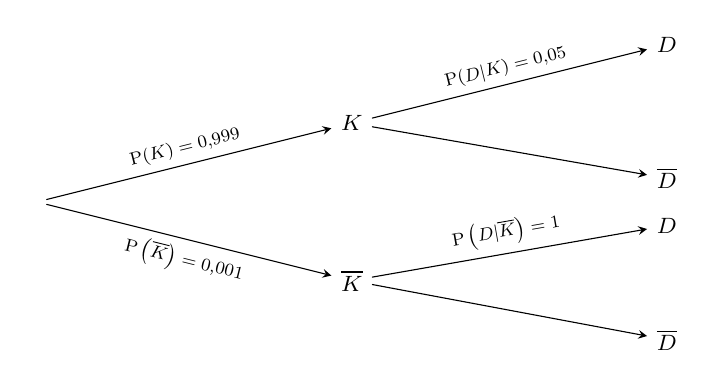
\begin{tikzpicture}[->,>=stealth,line join=round,line cap=round,font=\footnotesize,scale=1]
					\def\xmot{4}
					\def\xhai{8}
					\node (O) at (0,0){};
					\node (B) at (\xmot,1){$K$};
					\node (B1) at (\xmot,-1){$\overline{K}$};
					\node (BA) at (\xhai,2){$D$};
					\node (BA1) at (\xhai,0.3){$\overline{D}$};
					\node (B1A) at (\xhai,-0.3){$D$};
					\node (B1A1) at (\xhai,-1.75){$\overline{D}$};
					\foreach \x/\y/\p/\l in
					{
						O/B/above/$\mathrm{P}(K)=0{,}999$,
						B/BA/above/$\mathrm{P}(D|K)=0{,}05$,
						B/BA1//,
						O/B1/below/$\mathrm{P}\left(\overline{K}\right)=0{,}001$,
						B1/B1A/above/$\mathrm{P}\left(D|\overline{K}\right)=1$,
						B1/B1A1//
					}
					{
						\draw[->] (\x)--(\y)node[midway,\p,scale=0.8,sloped]{\l};
					}
				\end{tikzpicture}
			\end{center}
			\item Ta thấy rằng khả năng mắc bệnh của một người xét nghiệm có phản ứng dương tính chính là $\mathrm{P}\left(\overline{K}|D\right)$. Áp dụng công thức Bayes, ta có:
			\[\mathrm{P}\left(\overline{K}|D\right)=\dfrac{\mathrm{P}\left(\overline{K}\right)\cdot \mathrm{P}\left(D|\overline{K}\right)}{\mathrm{P}\left(\overline{K}\right)\cdot \mathrm{P}\left(D|\overline{K}\right) + \mathrm{P}(K)\cdot\mathrm{P}(D|K)}=\dfrac{0{,}001\cdot 1}{0{,}001\cdot 1 + 0{,}999 \cdot 0{,}05}\approx 1{,}96\%.\]
			Vậy xác suất mắc bệnh của một người xét nghiệm có phản ứng dương tính là $1{,}96\%$.
		\end{listEX}
	}
\end{vd}

\begin{vd}%[2D5H2-3]
	\immini{Một loại xét nghiệm nhanh SARS-CoV-2 cho
		kết quả dương tính với $76,2\%$ các ca thực sự
		nhiễm virus và kết quả âm tính với $99,1\%$ các
		ca thực sự không nhiễm virus (nguồn: https://
		tapchiyhocvietnam.vn/index.php/vmj/article/
		view/2124/1921). Giả sử tỉ lệ người nhiễm virus
		SARS-CoV-2 trong một cộng đồng là $1\%$.\\
		Một người làm xét nghiệm và nhận được kết quả dương tính.
		Tính xác suất người đó thực sự nhiễm virus (kết quả làm tròn đến hàng phần nghìn).
	}{\includegraphics[scale=0.5]{images/12-SGK-CTST-6-2-1.png}}
	\loigiai{
		Gọi $A$ là biến cố “Người làm xét nghiệm có kết quả dương tính” và $B$ là biến cố
		“Người làm xét nghiệm thực sự nhiễm virus”.\\
		Do xét nghiệm cho kết quả dương tính với $76,2\%$ các ca thực sự nhiễm virus nên $\mathrm{P}(A|B)=0{,}762$.\\
		Do xét nghiệm cho kết quả âm tính với $99,1\%$ các ca thực sự không nhiễm virus nên
		$\mathrm{P}(\overline{A}|\overline{B})=0{,}991$. Suy ra $$\mathrm{P}(A|\overline{B})=1-0{,}991=0{,}009.$$
		Do tỉ lệ người nhiễm virus trong cộng đồng là $1\%$ nên $\mathrm{P}(B)=0,01$ và $\mathrm{P}(\overline{B}) = 0,99$.
		Áp dụng công thức xác suất toàn phần, ta có xác suất người làm xét nghiệm có kết quả
		dương tính là $$\mathrm{P}(A)=\mathrm{P}(B)\mathrm{P}(A|B)+\mathrm{P}(\overline{B})\mathrm{P}(A|\overline{B})=0{,}01\cdot0{,}762+0{,}99\cdot0{,}009=0{,}01653.$$
		Xác suất một người thực sự nhiễm virus khi người đó có kết quả xét nghiệm dương tính
		là $\mathrm{P}(B|A)$. Ta có $$\mathrm{P}(B|A)=\dfrac{\mathrm{P}(B)\mathrm{P}(A|B)}{\mathrm{P}(A)}=\dfrac{0{,}01\cdot0{,}762}{0{,}01653}\approx0{,}461.$$}
\end{vd}
%----------------------------
\subsubsection{Bài tập áp dụng}
\begin{bt}%[2D5H2-3]
	Trong một kì sát hạch lái xe có $65 \%$ thí sinh nam. Biết rằng $80 \%$ thí sinh nam và $70\% $ thí sinh nữ đỗ kì sát hạch này.
	\begin{listEX}
		\item Tính tỉ lệ thí sinh đỗ kì sát hạch này.
		\item Chọn ngẫu nhiên một thí sinh đã đỗ kì sát hạch. Tính xác suất thí sinh đó là nữ.
	\end{listEX}
	\loigiai{
		\begin{listEX}
			\item Xét các biến cố sau
			\begin{itemize}
				\item $D$: \lq\lq  Thí sinh đỗ kì sát hạch\rq\rq
				\item $M$: \lq\lq  Thí sinh là nam giới\rq\rq\,
				\item $\overline{M}$: \lq\lq  Thí sinh là nữ giới\rq\rq\,
				\item $D|M$: \lq\lq  Thí sinh nam đỗ kì sát hạch\rq\rq\,
				\item $D|\overline{M}$: \lq\lq  Thí sinh nữ đỗ kì sát hạch\rq\rq\,.
			\end{itemize}
			Theo đề bài ta có
			\begin{center}
				$\mathrm{P}(M) =0{,}65$;  $\mathrm{P}(D|M) =0{,}8$; $\mathrm{P}(\overline{M}) =0{,}35$; $\mathrm{P}(D|\overline{M}) =0{,}7$.
			\end{center}
			Theo công thức xác suất toàn phần, ta có
			\begin{align*}
				\mathrm{P}(D) &= \mathrm{P}(M) \cdot \mathrm{P}(D|M) + \mathrm{P}(\overline{M}) \cdot \mathrm{P}(D|\overline{M}).
			\end{align*}
			Thay vào giá trị đã cho
			\begin{align*}
				\mathrm{P}(D) &= 0{,}65 \cdot 0{,}8 + 0{,}35 \cdot 0{,}7 \\
				&= 0{,}765.
			\end{align*}
			\item Xác suất một thí sinh đỗ là nữ\\
			Để tính xác suất này, ta sử dụng công thức Bayes
			\begin{align*}
				\mathrm{P}(\overline{M}|D) &= \dfrac{\mathrm{P}(D|\overline{M}) \cdot \mathrm{P}(\overline{M})}{\mathrm{P}(D)}.
			\end{align*}
			Thay vào giá trị đã cho và kết quả tính được ở trên
			\begin{align*}
				\mathrm{P}(\overline{M}|D) &= \dfrac{0{,}7 \cdot 0{,}35}{0{,}765} \\
				&\approx 0{,}321.
			\end{align*}
			Vậy, xác suất một thí sinh đỗ kì sát hạch là nữ là khoảng $0{,}321$, hay chấp nhận được là khoảng $32{,}1\%$.
		\end{listEX}
	}
\end{bt}
\begin{bt}%[2D5H2-3]
	Bạn Nam tham gia một gian hàng trò chơi dân gian trong hội xuân của trường. Trò chơi có hai lượt chơi. Xác suất để Nam thắng ở lượt chơi thứ nhất là $0{,}6$. Nếu Nam thắng ở lượt chơi thứ nhất thì xác suất Nam thắng ở lượt chơi thứ hai là $0{,}8 $. Ngược lại, nếu Nam thua ở lượt chơi thứ nhất thì xác suất Nam thắng ở lượt chơi thứ hai là $0{,}3$.
	\begin{listEX}
		\item Vẽ sơ đồ hình cây mô tả các khả năng xảy ra và xác suất tương ứng khi Nam tham gia trò chơi này.
		\item 	Biết Nam đã thắng ở lượt chơi thứ hai, tính xác suất Nam thắng ở lượt chơi thứ nhất.
	\end{listEX}
	\loigiai{
		\begin{listEX}
			\item Sơ đồ hình cây
			\begin{center}
				\begin{tikzpicture}[scale=.2,>=stealth]
					%-------------
					\tikzstyle{block} = [rectangle, draw, fill=cyan!20, rounded corners, text centered, text width = 10em, minimum height = 2em]
					%-------------
					\node (c1) [block] {Trò chơi};
					\node (c2) [block, above right = 3cm of c1]{Nam thắng lượt chơi thứ nhất};
					\node (c3) [block, below right= 3cm of c1]{Nam thua lượt chơi thứ nhất };
					\node (c4) [block,above right = 1.5cm of c2]{Nam thắng lượt chơi thứ hai};
					\node (c5) [block,below right = 1.5cm of c2]{Nam thua lượt chơi thứ hai};
					\node (c6) [block, above right =1.5cm of c3]{Nam thắng lượt chơi thứ hai};
					\node (c7) [block, below right = 1.5cm of c3]{Nam thua lượt chơi thứ hai};
					%--------------
					\draw[->] (c1.east) -- (c2.west);
					\draw[->] (c1.east) -- (c3.west);
					\draw[->] (c2.east) -- (c4.west);
					\draw[->] (c2.east) -- (c5.west);
					\draw[->] (c3.east) -- (c6.west);
					\draw[->] (c3.east) -- (c7.west);
					\draw ($(c1.east)!.5!(c2.west)$) node [below right=-.1]{\color{red}$\mathrm{P}(A) =0{,}6$};
					\draw ($(c1.east)!.5!(c3.west)$) node [above right=-.1]{\color{red}$\mathrm{P}(\overline{A}) =0{,}4$};
					\draw ($(c2.east)!.5!(c4.west)$) node [below right=-.1]{\color{red}$\mathrm{P}(B|A) =0{,}8$};
					\draw ($(c2.east)!.5!(c5.west)$) node [above right=-.1]{\color{red}$\mathrm{P}(\overline{B}|A) =0{,}2$};
					\draw ($(c3.east)!.5!(c6.west)$) node [below right=-.1]{\color{red}$\mathrm{P}(B|\overline{A}) =0{,}3$};
					\draw ($(c3.east)!.5!(c7.west)$) node [above right=-.1]{\color{red}$\mathrm{P}(\overline{B}|\overline{A}) =0{,}7$};
				\end{tikzpicture}
			\end{center}
			\item
			Công thức Bayes cho sự kiện $A$ và $B$ là $\mathrm{P}(A | B)=\dfrac{\mathrm{P}(B | A) \cdot \mathrm{P}(A)}{\mathrm{P}(B)}	$.\\
			Trong đó
			\begin{itemize}
				\item $A$ là Nam thắng ở lượt chơi thứ nhất.
				\item $B$ là Nam thắng ở lượt chơi thứ hai.
				\item $\mathrm{P}(A)$: Xác suất Nam thắng ở lượt chơi thứ nhất $0{,}6$.
				\item $\mathrm{P}(B | A)$: Xác suất Nam thắng ở lượt chơi thứ hai khi đã thắng ở lượt chơi thứ nhất $0{,}8$.
				\item $\mathrm{P}(B | \overline{A})$: Xác suất Nam thắng ở lượt chơi thứ hai khi đã thua ở lượt chơi thứ nhất $0.3$.
			\end{itemize}
			Công thức Bayes:
			$$
			\begin{aligned}[t]
				\mathrm{P}(A | B)&=\dfrac{\mathrm{P}(B | A) \cdot \mathrm{P}(A)}{\mathrm{P}(B | A) \cdot \mathrm{P}(A)+\mathrm{P}(B | \overline{A}) \cdot \mathrm{P}(\overline{A})} \\
				& =\dfrac{0{,}8 \cdot 0{,}6}{0{,}8 \cdot 0{,}6+0{,}3 \cdot 0{,}4} \\
				& = \dfrac{0{,}48}{0{,}48+0{,}12} \\
				& = \dfrac{0{,}48}{0{,}6} \\
				& = 0{,}8.
			\end{aligned}
			$$
			Vậy, xác suất Nam thắng ở lượt chơi thứ nhất khi đã thắng ở lượt chơi thứ hai là khoảng $0{,}8$ hoặc $80 \%$.
		\end{listEX}
	}
\end{bt}

\begin{bt}%[2D5H2-3]
	Năm $2001$, Cộng đồng châu Âu có làm một đợt kiểm tra rất rộng rãi các con bò để phát hiện những con bị bệnh bò điên. Không có xét nghiệm nào cho kết quả chính xác $100 \%$. Một loại xét nghiệm, mà ở đây ta gọi là xét nghiệm $A$ cho kết quả như sau: khi con bò bị bệnh bò điên thì xác suất để có phản ứng dương tính trong xét nghiệm A là $70 \%$ còn khi con bò không bị bệnh thì xác suất để có phản ứng dương tính trong xét nghiệm $A$ là $10 \%$. Biết rằng tỉ lệ bò bị mắc bệnh bò điên ở Hà Lan là $13$ con trên $1~000~000$ con \textit{(Nguồn: F. M. Dekking et al., Amodern introduction to probability and statistics Understanding why and how, Springer, $2005$)}. Hỏi khi một con bò ở Hà Lan có phản ứng dương tính với xét nghiệm $A$ thì xác suất để nó bị mắc bệnh bò điên là bao nhiêu?
	\loigiai{
		Xét hai biến cố\\
		$N$: \lq\lq  Con bò được chọn bị nhiễm bệnh\rq\rq.\\
		$D$: \lq\lq  Con bò được chọn có phản ứng dương tính\rq\rq.\\
		Khi đó, ta có\\
		\[\mathrm{P}(N)=\dfrac{13}{1 000 000}=0{,}000013; \qquad \mathrm{P}(\overline{N})=1-\mathrm{P}(N)=0{,}999987;\]
		\[\mathrm{P}(D|N)=70\%=0{,}7; \qquad \mathrm{P}(D|\overline{N})=10\%=0{,}1.\]
		Áp dụng công thức Bayes, ta có\\
		$\mathrm{P}(N|D)=\dfrac{\mathrm{P}(D|N) \cdot \mathrm{P}(N)}{\mathrm{P}(N) \cdot \mathrm{P}(D|N)+\mathrm{P}(\overline{N})\mathrm{P}(D|\overline{N})}=\dfrac{0{,}7 \cdot 0{,}000013}{0{,}7 \cdot 0{,}000013+0{,}1 \cdot 0{,}999987}\approx 0{,}009\%$.
	}
\end{bt}
\begin{bt}%[2D5H2-3]
	\immini{Khi phát hiện một vật thể bay, xác suất một hệ thống radar phát
		cảnh báo là $0,9$ nếu vật thể bay đó là mục tiêu thật và là $0,05$
		nếu đó là mục tiêu giả. Có $99\%$ các vật thể bay là mục tiêu giả.
		Biết rằng hệ thống radar đang phát cảnh báo khi phát hiện một
		vật thể bay. Tính xác suất vật thể đó là mục tiêu thật.}{\includegraphics[scale=0.7]{images/12-SGK-CTST-6-2-4.png}}	\loigiai{Gọi $ A $ là biến cố \lq\lq  Hệ thống radar phát cảnh báo\rq\rq \, và $ B $ là biến cố \lq\lq  Vật thể bay là mục tiêu thật\rq\rq.\\
		Do xác suất một hệ thống radar cảnh báo nếu vật thể bay là mục tiêu thật là $ 0,9 $ nên $ \mathrm{P}(A|B)=0,9 $. \\
		Do xác suất một hệ thống radar cảnh báo nếu vật thể bay là mục tiêu giả là $ 0,05 $ nên $ \mathrm{P}(A|\overline{B})=0,05 $. \\
		Do có $ 99\% $ các vật thể bay là mục tiêu giả nên $ \mathrm{P}(\overline{B})=0,99 $ và $ \mathrm{P}(B)= 0,01$.\\
		Áp dụng công thức xác suất toàn phần, ta có xác suất để hệ thống radar phát cảnh báo là
		$$ \mathrm{P}(A)=\mathrm{P}(B)\mathrm{P}(A|B)+\mathrm{P}(\overline{B})\mathrm{P}(A|\overline{B})=0,01 \cdot 0,9+0,99 \cdot 0,05= 0,0585$$
		Xác suất vật bay là mục tiêu thật khi hệ thống radar đang phát cảnh báo là $ \mathrm{P}(B|A) $. Ta có
		$$ \mathrm{P}(B|A)=\dfrac{\mathrm{P}(B)\mathrm{P}(A|B)}{\mathrm{P}(A)}=\dfrac{0,01 \cdot 0,9}{0,0585}=\dfrac{2}{13}. $$}
\end{bt}
\begin{bt}%[2D5H2-3]
	Trong một kho rượu có 30\% là rượu loại I. Chọn ngẫu nhiên một chai rượu đưa cho ông Tùng, một người sành rượu, để nếm thử. Biết rằng, một chai rượu loại I có xác suất 0{,}9 để ông Tùng xác nhận là loại I; một chai rượu không phải loại I có xác suất 0{,}95 để ông Tùng xác nhận đây không phải là loại I. Sau khi nếm, ông Tùng xác nhận đây là rượu loại I. Tính xác suất để chai rượu đúng là rượu loại I.
	\loigiai{Xét biến cố $A$: ``Chai rượu đó là chai rượu loại I''. Xét biến cố $B$: ``Ông Tùng xác nhận chai rượu đó là rượu loại I''.\\
		Ta cần tính $\mathrm{P}(A\mid B)$.
		Áp dụng công thức Bayes
		$$\mathrm{P}(A\mid B) = \dfrac{\mathrm{P}(A)\cdot \mathrm{P}(B\mid A)}{\mathrm{P}(A)\cdot \mathrm{P}(B\mid A) + \mathrm{P}(\overline{A})\cdot \mathrm{P}(B \mid \overline{A})}.$$
		\begin{itemize}
			\item Tính $P\mathrm{P}(A)$: Đây là chai rượu đó là chai rượu loại I. Vậy $\mathrm{P}(A)=0{,}3$.
			\item Tính $\mathrm{P}(\overline{A})$: $\mathrm{P}(\overline{A})=1-\mathrm{P}(A)=0{,}7$.
			\item Tính $\mathrm{P}(B \mid A)$: Đây là xác suất ông Tùng xác nhận đúng một chai rượu loại I là một chai rượu loại I. Vậy $\mathrm{P}(B \mid A)=0{,}9$.
			\item Tính $\mathrm{P}(B \mid \overline{A})$: Đây là xác suất ông Tùng xác nhận sai một chai rượu không phải loại I là một chai rượu loại I. Vậy $\mathrm{P}(B \mid \overline{A})=1-0{,}95=0{,}05$.
		\end{itemize}
		Vậy ta có
		$$\mathrm{P}(A\mid B) = \dfrac{\mathrm{P}(A)\cdot \mathrm{P}(B\mid A)}{\mathrm{P}(A)\cdot \mathrm{P}(B\mid A) + \mathrm{P}(\overline{A})\cdot \mathrm{P}(B \mid \overline{A})}=\dfrac{0{,}3\cdot 0{,}9}{0{,}3\cdot 0{,}9+0{,}7\cdot 0{,}05}=\dfrac{270}{277}\approx 0{,}8852.$$
		Vậy xác suất để chai rượu mà ông Tùng xác nhận là rượu loại I đúng là rượu loại I là khoảng $0{,}8852$.}
\end{bt}
\begin{bt}%[2D5H2-3]
	Một loại linh kiện do hai nhà máy số I, số II cùng sản xuất. Tỉ lệ phế phẩm của các nhà máy I, II lần lượt là $4\%$; $3\%$. Trong một lô linh kiện để lẫn lộn $80$ sản phẩm của nhà máy số I và $120$ sản phẩm của nhà máy số II. Một khách hàng lấy ngẫu nhiên một linh liện từ lô hàng đó.
	\begin{listEX}
		\item Tính xác suất để linh kiện được lấy ra là linh kiện tốt.
		\item Giả sử linh kiện được lấy ra là linh kiện phế phẩm. Xác suất linh kiện đó do nhà máy nào sản xuất là cao nhất?
	\end{listEX}
	\loigiai{
		\begin{listEX}
			\item Xét các biến cố
			\begin{itemize}
				\item $A$: \lq\lq  Linh kiện lấy ra là linh kiện tốt\rq\rq.
				\item $B_1$: \lq\lq  Linh kiện lấy ra là linh kiện từ nhà máy số I\rq\rq.
				\item $B_2$: \lq\lq  Linh kiện lấy ra là linh kiện từ nhà máy số II\rq\rq.
			\end{itemize}
			Theo đề bài, ta có
			\begin{listEX}[2]
				\item[] $\mathrm{P}(A|B_1) =1 - 0{,}04 = 0{,}96$.
				\item[] $\mathrm{P}\left(A|B_2\right) = 1-0{,}03 = 0{,}97$.
				\item[] $\mathrm{P}(B_1)=\dfrac{80}{200}=0{,}4$.
				\item[] $\mathrm{P}\left(B_2\right) = \dfrac{120}{200}=0{,}6$.
			\end{listEX}
			Khi đó áp dụng công thức xác suất toàn phần, ta có
			\[\mathrm{P}(A) = \mathrm{P}(A|B_1)\cdot \mathrm{P}(B_1) + \mathrm{P}\left(A|B_2\right)\cdot\mathrm{P}\left(B_2\right)=0{,}96\cdot 0{,}4 + 0{,}97\cdot 0{,}6=0{,}966.\]
			\item Ta có $\mathrm{P}\left(\overline{A}\right)=1-\mathrm{P}(A) = 0{,}034$.\\
			Áp dụng công thức Bayes, ta có
			\begin{itemize}
				\item $\mathrm{P}\left(B_1|\overline{A}\right)=\dfrac{\mathrm{P}\left(\overline{A}|B_1\right)\cdot \mathrm{P}(B_1)}{\mathrm{P}\left(\overline{A}\right)} = \dfrac{0{,}04\cdot 0{,}4}{0{,}034} = \dfrac{8}{17}\approx 0{,}048$.
				\item $\mathrm{P}\left(B_2|\overline{A}\right)=\dfrac{\mathrm{P}\left(\overline{A}|B_2\right)\cdot \mathrm{P}(B_2)}{\mathrm{P}\left(\overline{A}\right)} = \dfrac{0{,}03\cdot 0{,}6}{0{,}034} = \dfrac{8}{167}\approx 0{,}054$.
			\end{itemize}
			Vậy với điều kiện linh kiện lấy ra là linh kiện phế phẩm thì xác suất linh kiện đó do nhà máy II sản xuất là cao nhất.
		\end{listEX}
	}
\end{bt}
\begin{bt}%[2D5V2-3]
	Một nghiên cứu đã chỉ ra rằng tỉ lệ người bị lao phổi trong nhóm $X$ những người mắc phải hội chứng suy giảm miễn dịch $ {H}$ là $15{,}2 \%$. Kết quả nghiên cứu về một số triệu chứng lâm sàng như có ho trong vòng bốn tuần, hoặc có bị sốt trong vòng bốn tuần, hoặc ra mồ hôi ban đêm từ ba tuần trở lên của nhóm $X$ cho thấy.
	\begin{itemize}
		\item Trong số những người mắc bệnh lao phổi, có $93{,}2 \%$ trường hợp có ít nhất một triệu chứng;
		\item Trong số những người không mắc bệnh lao phổi, có $35{,}8 \%$ trường hợp không có triệu chứng nào.
	\end{itemize}
	Nếu bác sĩ gặp một bệnh nhân thuộc nhóm $X$ và bệnh nhân đó có ít nhất một triệu chứng trên thì xác suất bệnh nhân này mắc bệnh lao phổi là bao nhiêu?
	\loigiai{
		Gọi $A$ là biến cố \lq\lq  Người bị lao phổi\lq\lq .\\
		$\overline{A}$ là biến cố \lq\lq  Người không mắc lao phổi\lq\lq .\\
		$B$ là biến cố \lq\lq  Những người có ít nhất một triệu chứng\rq\rq.\\
		$\overline{B}$ là biến cố \lq\lq  Những người không có triệu chứng\rq\rq.\\
		Ta có $\mathrm{P}(A)=0{,}152$. \\
		Khi đó, xác suất những người không mắc lao phổi là $$\mathrm{P}\left(\overline{A}\right)=1-0{,}152=0{,}848.$$
		Ta có xác suất những người có ít một triệu chứng trong những người mắc lao phổi là $$\mathrm{P}\left(B|A\right)=0{,}932.$$
		Khi đó, xác suất những người không có triệu chứng trong những người mắc lao phổi là  $$\mathrm{P}\left(\overline{B}|A\right)=1-0{,}932=0{,}068.$$
		Mặt khác, ta có xác suất những người không có triệu chứng  $$\mathrm{P}\left(\overline{B}|\overline{A}\right)=0{,}358.$$
		Khi đó, xác suất những người có ít nhất một triệu chứng trong những người không mắc bệnh lao phổi là $$\mathrm{P}\left(B|\overline{A}\right)=1-0{,}358=0{,}642.$$
		Ta có $\mathrm{P}(B)=\mathrm{P}\left(B|A\right)\cdot \mathrm{P}(A)+\mathrm{P}\left(B|\overline{A}\right)\cdot \mathrm{P}\left(\overline{A}\right)=0{,}932\cdot 0{,}152+0{,}642\cdot 0{,}848=0{,}68608$.\\
		Theo công thức Bayes, ta có $\mathrm{P}(A|B)=\dfrac{\mathrm{P}(A)\cdot\mathrm{P}\left(B|A\right)}{\mathrm{P}(B)}=\dfrac{0{,}152\cdot 0{,}932}{0{,}68608}\approx 0{,}2065$.
	}
\end{bt}
\begin{bt}%[2D5V2-3]
	Có hai hộp đựng các viên bi cùng kích thước và khối lượng. Hộp thứ nhất chứa $5$ viên bi đỏ và $5$ viên bi xanh, hộp thứ hai chứa $6$ viên bi đỏ và $4$ viên bi xanh. Lấy ngẫu nhiên một viên bi từ hộp thứ nhất chuyển sang hộp thứ hai, sau đó lấy ra ngẫu nhiên một viên bi từ hộp thứ hai (giả sử viên bi được lấy ra từ hộp thứ hai là bi đỏ). Tính xác suất viên bi đỏ đó là của hộp thứ nhất.
	\loigiai{
		Gọi $A$ là biến cố \lq\lq  Viên bi được lấy ra từ hộp thứ hai là bi đỏ\rq\rq.\\
		$B$ là biến cố \lq\lq  Viên bi được lấy ra từ hộp thứ nhất chuyển sang hộp thứ hai là viên bi đỏ\rq\rq.\\
		$\overline{B}$ là biến cố \lq\lq  Viên bi được lấy ra từ hộp thứ nhất chuyển sang hộp thứ hai là bi xanh\rq\rq.\\
		Ta có $\mathrm{P}(B)=\dfrac{5}{10}=\dfrac{1}{2}$; $\mathrm{P}(\overline{B})=\dfrac{5}{10}=\dfrac{1}{2}$.\\
		Nếu viên bi được lấy ra từ hộp thứ nhất chuyển sang hộp thứ hai là bi đỏ thì sau khi chuyển, hộp thứ hai có $7$ bi đỏ và $4$ bi xanh. Do đó $\mathrm{P}(A\mid B) =\dfrac{7}{11}$.\\
		Nếu viên bi được lấy ra từ hộp thứ nhất chuyển sang hộp thứ hai là bi xanh thì sau khi chuyển, hộp thứ hai có $6$ bi đỏ và $5$ bi xanh. Do đó $\mathrm{P}(A\mid \overline{B})=\dfrac{6}{11}$.\\
		Áp dụng công thức xác suất toàn phần ta có
		$$\mathrm{P})(A) = \mathrm{P}(B) \cdot \mathrm{P}(A\mid B) + \mathrm{P}(\overline{B}) \cdot \mathrm{P}(A\mid \overline{B}) = \dfrac{1}{2} \cdot \dfrac{7}{11} + \dfrac{1}{2}\cdot \dfrac{6}{11} = \dfrac{13}{22}.$$
		Xác suất viên bi được lấy ra từ hộp thứ nhất chuyển sang hộp thứ hai là viên bi đỏ khi biết viên bi lấy ra từ hộp thứ hai là bi đỏ là
		$$\mathrm{P}(B\mid A) =\dfrac{\mathrm{P}(B) \cdot \mathrm{P}(A\mid B)}{\mathrm{P}(A)} = \dfrac{\dfrac{1}{2} \cdot \dfrac{7}{11}}{\dfrac{13}{22}} = \dfrac{7}{13}.$$
		Vì khi viên bi lấy sang hộp thứ II là bi đỏ thì hộp II có $7$ bi đỏ, do vậy xác suất viên bi đỏ lấy ra là của hộp thứ nhất là $\dfrac{1}{7}\cdot\dfrac{7}{13}=\dfrac{1}{13}$.
	}
\end{bt}
\begin{bt}%[2D5V2-3]
	Có hai chiếc hộp, hộp I có $5$ viên bi màu trắng và $5$ viên bi màu đen; hộp II có $6$ viên bi màu trắng và $4$ viên bi màu đen. Các viên bi có cùng kích thước và khối lượng. Lấy ngẫu nhiên đồng thời hai viên bi từ hộp I bỏ sang hộp II. Sau đó lấy ngẫu nhiên một viên bi từ hộp II.
	\begin{listEX}
		\item Tính xác suất để viên bi được lấy ra là viên bi màu trắng.
		\item Giả sử viên bi được lấy ra là viên bi màu trắng. Tính xác suất viên bi màu trắng đó thuộc hộp I.
	\end{listEX}
	\loigiai{
		\begin{listEX}
			\item Xét các biến cố
			\begin{itemize}
				\item $A$: \lq\lq  Viên bi lấy ra là viên màu trắng\rq\rq.
				\item $B_1$: \lq\lq  2 viên bi lấy ra từ hộp I có màu trắng\rq\rq.
				\item $B_2$: \lq\lq  2 viên bi lấy ra từ hộp I có màu đen\rq\rq.
				\item $B_3$: \lq\lq  2 viên bi lấy ra từ hộp I có cả hai màu đen trắng\rq\rq.
			\end{itemize}
			Ta có
			\[\mathrm{P}(B_1) = \dfrac{\mathrm{C}^2_{5}}{\mathrm{C}^2_{10}}=\dfrac{2}{9};\quad
			\mathrm{P}(B_2) = \dfrac{\mathrm{C}^2_5}{\mathrm{C}^2_{10}}=\dfrac{2}{9};\quad
			\mathrm{P}(B_3) = \dfrac{\mathrm{C}^1_5\cdot\mathrm{C}^1_5}{\mathrm{C}^2_{10}}=\dfrac{5}{9}.
			\]
			Áp dụng công thức xác suất toàn phần, ta có
			\allowdisplaybreaks
			\begin{eqnarray*}
				\mathrm{P}(A)
				&=& \mathrm{P}(A|B_1)\cdot \mathrm{P}(B_1) + \mathrm{P}(A|B_2)\cdot\mathrm{P}(B_2) + \mathrm{P}(A|B_3)\cdot\mathrm{P}(B_3)\\
				&=& \dfrac{8}{12}\cdot \dfrac{2}{9} + \dfrac{6}{12}\cdot \dfrac{2}{9} + \dfrac{7}{12}\cdot \dfrac{5}{9}\\
				&=& \dfrac{7}{12}.
			\end{eqnarray*}
			\item Gọi $C$ là biến cố \lq\lq  Viên bi được lấy ra là viên màu trắng thuộc hộp I\rq\rq.\\
			Ta cần tính $\mathrm{P}(C|A)$. \\
			Khi $B_1$ xảy ra, hộp II có $2$ viên bi trắng là từ hộp I nên $P(C|B_1)=\dfrac{2}{12}$.\\
			Khi $B_2$ xảy ra, hộp II không có viên bi trắng nào là từ hộp I nên $P(C|B_2)=0$.\\
			Khi $B_3$ xảy ra, hộp II có $1$ viên bi trắng là từ hộp I nên $P(C|B_3)=\dfrac{1}{12}$.\\
			Do đó, ta có
			\allowdisplaybreaks
			\begin{eqnarray*}
				\mathrm{P}(C) &=& \mathrm{P}(C|B_1)\cdot \mathrm{P}(B_1) + \mathrm{P}(C|B_2)\cdot \mathrm{P}(B_2) + \mathrm{P}(C|B_3)\cdot \mathrm{P}(B_3)\\
				&=& \dfrac{2}{12}\cdot \dfrac{2}{9} + 0 + \dfrac{1}{12}\cdot \dfrac{5}{9}\\
				&=& \dfrac{1}{12}.
			\end{eqnarray*}
			Đồng thời vì khi $C$ xảy ra thì $A$ cũng xảy ra nên $\mathrm{P}(A|C)=1$.\\
			Áp dụng công thức Bayes, ta có
			$$\mathrm{P}(C|A) = \dfrac{\mathrm{P}(C)\cdot \mathrm{P}(A|C)}{\mathrm{P}(A)} 
				= \dfrac{\dfrac{1}{12}\cdot 1}{\dfrac{7}{12}} = \dfrac{1}{7}.$$
		\end{listEX}
	}
\end{bt}
%===================
